% !TEX program = xelatex
\documentclass[12pt,a4paper]{article}

\usepackage{fontspec}
\usepackage{polyglossia}
\setmainlanguage{greek}
\setotherlanguage{english}
\setmainfont[Script=Greek]{DejaVu Serif}
\setsansfont[Script=Greek]{DejaVu Sans}
\setmonofont[Script=Greek]{DejaVu Sans Mono}
\newfontfamily\greekfonttt[Script=Greek]{DejaVu Sans Mono}

\usepackage[a4paper, margin=2.35cm]{geometry}
\usepackage{amsmath, amssymb}
\usepackage{booktabs}
\usepackage{array}
\usepackage{longtable}
\usepackage{graphicx}
\usepackage{float}
\usepackage{caption}
\usepackage[hidelinks]{hyperref}
\usepackage{enumitem}
\usepackage{parskip}
\usepackage{xcolor}
\usepackage{fancyhdr}

\pagestyle{fancy}
\fancyhf{}
\lhead{Τεχνικές και Οργάνωση Ελέγχου Ποιότητας}
\rhead{Explanatory Report}
\cfoot{\thepage}
\setlength{\headheight}{14.5pt}

\captionsetup{font=small, labelfont=bf}
\graphicspath{{./}}
\renewcommand{\arraystretch}{1.22}
\setlength{\parindent}{0pt}
\sloppy

\newcommand{\code}[1]{\texttt{\textenglish{#1}}}
\newcommand{\Pa}{P_{\!a}}
\newcommand{\AOQ}{\textenglish{AOQ}}
\newcommand{\AOQL}{\textenglish{AOQL}}
\newcommand{\ATI}{\textenglish{ATI}}
\newcommand{\ASN}{\textenglish{ASN}}
\newcommand{\AQL}{\textenglish{AQL}}
\newcommand{\OC}{\textenglish{OC}}

\title{
    \textbf{Τεχνικές και Οργάνωση Ελέγχου Ποιότητας}\\[0.25cm]
    \Large Αναλυτικό Explanatory Report\\[0.15cm]
    \large Δειγματοληπτικός έλεγχος αποδοχής και διαγράμματα ελέγχου
}
\author{Τσακιρίδης}
\date{\today}

\begin{document}

\maketitle
\thispagestyle{fancy}

\begin{abstract}
Το παρόν report είναι γραμμένο σαν επεξηγηματικό μάθημα. Δεν περιορίζεται στο
να δώσει τα τελικά αριθμητικά αποτελέσματα, αλλά εξηγεί πρώτα τι ζητά κάθε
ερώτημα, ποια θεωρία χρειάζεται για να το καταλάβουμε και έπειτα πώς
προκύπτει η λύση βήμα προς βήμα. Η εργασία χωρίζεται σε δύο μέρη. Στο Μέρος Α
μελετάται δειγματοληπτικός έλεγχος αποδοχής παρτίδων με διαλογή. Στο Μέρος Β
μελετώνται διαγράμματα ελέγχου μέσης τιμής και τυπικής απόκλισης για την τάση
εξόδου ηλεκτρονικών τροφοδοτικών.
\end{abstract}

\tableofcontents
\newpage

%=============================================================================
\section*{Πώς να διαβαστεί αυτό το report}
\addcontentsline{toc}{section}{Πώς να διαβαστεί αυτό το report}
%=============================================================================

Αυτό το κείμενο απευθύνεται σε κάποιον που δεν έχει ακόμη άνεση με τις έννοιες
του μαθήματος. Για αυτόν τον λόγο κάθε ερώτημα έχει τρεις διακριτές φάσεις:

\begin{enumerate}
    \item \textbf{Τι ζητάει το ερώτημα.} Εδώ μεταφράζουμε την εκφώνηση σε απλή
    γλώσσα.
    \item \textbf{Θεωρητικό υπόβαθρο.} Εξηγούμε τις έννοιες και τους τύπους
    που χρειάζονται, πριν τους χρησιμοποιήσουμε.
    \item \textbf{Λύση βήμα προς βήμα.} Παίρνουμε τα δεδομένα της εργασίας,
    εφαρμόζουμε τους τύπους και παρουσιάζουμε το τελικό αποτέλεσμα.
\end{enumerate}

Οι υπολογισμοί έγιναν με Python, στο αρχείο \code{toep\_solution.py}. Τα
αριθμητικά αποτελέσματα και τα γραφήματα έχουν αντιγραφεί στον παρόντα φάκελο,
ώστε το report να μπορεί να διαβαστεί αυτόνομα.

\newpage

%=============================================================================
\section{Αρχικά δεδομένα}
%=============================================================================

\subsection{Γιατί ξεκινάμε από τα δεδομένα}

Πριν λύσουμε οποιαδήποτε άσκηση ποιοτικού ελέγχου, πρέπει να καταλάβουμε τι
σημαίνει κάθε αριθμός. Στις ασκήσεις ΤΟΕΠ οι παράμετροι δεν είναι απλώς
νούμερα. Συνδέονται με αποφάσεις: αποδεχόμαστε ή απορρίπτουμε μια παρτίδα,
σταματάμε ή όχι μια παραγωγική διαδικασία, πληρώνουμε κόστος ελέγχου ή κόστος
κακής ποιότητας.

\subsection{Δεδομένα Μέρους Α}

Στο πρώτο μέρος έχουμε παρτίδες εξαρτημάτων μεγέθους \(N=600\). Η επιχείρηση
δεν θέλει να ελέγχει πάντα όλα τα εξαρτήματα, γιατί ο έλεγχος έχει κόστος.
Θέλει λοιπόν να πάρει ένα δείγμα και, με βάση τα ελαττωματικά που θα βρει στο
δείγμα, να αποφασίσει αν θα δεχτεί ή θα απορρίψει την παρτίδα.

\begin{table}[H]
\centering
\caption{Δεδομένα για τον δειγματοληπτικό έλεγχο αποδοχής.}
\small
\begin{tabular}{>{\centering\arraybackslash}p{2.0cm}>{\centering\arraybackslash}p{2.0cm}p{9.3cm}}
\toprule
\textbf{Σύμβολο} & \textbf{Τιμή} & \textbf{Ερμηνεία} \\
\midrule
\(N\) & 600 & Πλήθος εξαρτημάτων σε κάθε παρτίδα \\
\(c_i\) & 6 € & Κόστος ελέγχου για κάθε εξάρτημα \\
\(c_d\) & 400 € & Κόστος για κάθε ελαττωματικό που διαφεύγει \\
\(p_1\) & 0,0065 & Αποδεκτή στάθμη ποιότητας, δηλαδή ΑΣΠ \\
\(\alpha\) & 0,03 & Μέγιστος επιτρεπτός κίνδυνος παραγωγού \\
\(\beta\) & 0,10 & Μέγιστος επιτρεπτός κίνδυνος πελάτη \\
\(p_2=7p_1\) & 0,0455 & Κακή στάθμη ποιότητας που θέλουμε να απορρίπτεται συχνά \\
\(p_L\) & 0,004 & Κάτω όριο για το τυχαίο ποσοστό ελαττωματικών στο Ερώτημα Α4 \\
\(p_U\) & 0,060 & Άνω όριο για το τυχαίο ποσοστό ελαττωματικών στο Ερώτημα Α4 \\
\bottomrule
\end{tabular}
\end{table}

Το \(p_1=0{,}0065\) σημαίνει ότι μια ``καλή'' παρτίδα έχει περίπου 0,65\%
ελαττωματικά. Το \(p_2=0{,}0455\) σημαίνει ότι μια ``κακή'' παρτίδα έχει
περίπου 4,55\% ελαττωματικά. Η εργασία μάς ζητά να σχεδιάσουμε σχήματα ελέγχου
που να ξεχωρίζουν, όσο γίνεται, αυτές τις δύο περιπτώσεις.

\subsection{Δεδομένα Μέρους Β}

Στο δεύτερο μέρος δεν ελέγχουμε παρτίδες εξαρτημάτων, αλλά παρακολουθούμε μια
παραγωγική διαδικασία. Το προϊόν είναι ηλεκτρονικό τροφοδοτικό και το κρίσιμο
χαρακτηριστικό ποιότητας είναι η τάση εξόδου.

\begin{table}[H]
\centering
\caption{Δεδομένα για τα διαγράμματα ελέγχου.}
\small
\begin{tabular}{>{\centering\arraybackslash}p{2.0cm}>{\centering\arraybackslash}p{2.0cm}p{9.3cm}}
\toprule
\textbf{Σύμβολο} & \textbf{Τιμή} & \textbf{Ερμηνεία} \\
\midrule
\(\mu_0\) & 9 V & Στόχος της μέσης τάσης \\
\(A\) & 0,10 V & Ημιπλάτος ορίων προδιαγραφών \\
\(\sigma\) & 0,035 V & Τυπική απόκλιση όταν η διαδικασία είναι κανονική \\
\(K\) & 21 € & Κόστος κακής ποιότητας ανά ελαττωματικό τροφοδοτικό \\
\(\Delta\) & 0,06 V & Πιθανή μεταβολή της μέσης τάσης \\
\(k\) & 2,5 & Πόσες τυπικές αποκλίσεις μπαίνουν τα όρια ελέγχου \\
\(n\) & 5 & Μέγεθος δείγματος κάθε ώρα \\
\bottomrule
\end{tabular}
\end{table}

Τα όρια προδιαγραφών είναι:
\[
    9\pm A = 9\pm 0{,}10.
\]

Άρα ένα τροφοδοτικό θεωρείται αποδεκτό αν η τάση του βρίσκεται μεταξύ:
\[
    8{,}90 \text{ V και } 9{,}10 \text{ V}.
\]

\newpage

%=============================================================================
\section{Μέρος Α: Δειγματοληπτικός έλεγχος αποδοχής}
%=============================================================================

\subsection{Γενική ιδέα του Μέρους Α}

Στο Μέρος Α η επιχείρηση παραλαμβάνει παρτίδες από έναν προμηθευτή. Κάθε
παρτίδα έχει \(600\) εξαρτήματα. Κάποια από αυτά μπορεί να είναι ελαττωματικά.

Η απλή λύση θα ήταν να ελέγχονται πάντα και τα 600 εξαρτήματα. Αυτό όμως είναι
ακριβό. Η άλλη ακραία λύση θα ήταν να μη γίνεται κανένας έλεγχος. Αυτό όμως
είναι επικίνδυνο, γιατί ελαττωματικά εξαρτήματα μπορεί να περάσουν στην
παραγωγή και να προκαλέσουν πολύ μεγαλύτερο κόστος αργότερα.

Ο δειγματοληπτικός έλεγχος αποδοχής είναι ένας συμβιβασμός. Ελέγχουμε ένα
μέρος της παρτίδας και αποφασίζουμε για όλη την παρτίδα.

\subsection{Τι σημαίνει ``με διαλογή''}

Η εκφώνηση λέει ότι έχουμε έλεγχο αποδοχής με διαλογή. Αυτό σημαίνει:

\begin{itemize}
    \item Αν η παρτίδα γίνει αποδεκτή, κρατάμε την παρτίδα, αλλά τα
    ελαττωματικά που βρέθηκαν μέσα στο δείγμα επιστρέφονται για επισκευή.
    \item Αν η παρτίδα απορριφθεί, τότε ελέγχονται και τα 600 εξαρτήματα.
    Όσα ελαττωματικά βρεθούν επιστρέφονται για επισκευή.
\end{itemize}

Άρα, όταν μια παρτίδα απορρίπτεται, στο τέλος η εξερχόμενη ποιότητα είναι πολύ
καλή, γιατί η παρτίδα έχει ελεγχθεί 100\%. Τα ελαττωματικά που μπορούν να
διαφύγουν υπάρχουν μόνο στις παρτίδες που γίνονται αποδεκτές.

%-----------------------------------------------------------------------------
\subsection{Ερώτημα Α1: Απλό δειγματοληπτικό σχήμα}
%-----------------------------------------------------------------------------

\subsubsection*{Τι ζητάει το ερώτημα}

Το πρώτο ερώτημα ζητά να βρούμε ένα απλό δειγματοληπτικό σχήμα. Απλό σχήμα
σημαίνει ότι παίρνουμε ένα μόνο δείγμα από την παρτίδα.

Ένα απλό σχήμα περιγράφεται από δύο αριθμούς:
\[
    (n,c).
\]

Ο αριθμός \(n\) είναι το μέγεθος του δείγματος. Ο αριθμός \(c\) είναι ο
αριθμός αποδοχής. Η απόφαση παίρνεται ως εξής:

\begin{itemize}
    \item Αν στο δείγμα βρεθούν το πολύ \(c\) ελαττωματικά, η παρτίδα γίνεται
    αποδεκτή.
    \item Αν στο δείγμα βρεθούν περισσότερα από \(c\) ελαττωματικά, η παρτίδα
    απορρίπτεται και ελέγχεται 100\%.
\end{itemize}

Το ερώτημα θέλει το σχήμα να ικανοποιεί τρεις απαιτήσεις:

\begin{enumerate}
    \item Να προστατεύει τον παραγωγό στις καλές παρτίδες.
    \item Να προστατεύει τον πελάτη στις κακές παρτίδες.
    \item Να έχει αρκετά χαμηλό όριο μέσης εξερχόμενης ποιότητας.
\end{enumerate}

\subsubsection*{Θεωρητικό υπόβαθρο}

Αν το πραγματικό ποσοστό ελαττωματικών μιας παρτίδας είναι \(p\), τότε ο
αριθμός ελαττωματικών που θα βρούμε σε δείγμα μεγέθους \(n\) ακολουθεί περίπου
διωνυμική κατανομή:
\[
    X\sim B(n,p).
\]

Η πιθανότητα να αποδεχτούμε την παρτίδα είναι η πιθανότητα να βρούμε το πολύ
\(c\) ελαττωματικά:
\[
    \Pa(p)=P(X\le c).
\]

Αναλυτικά:
\[
    \Pa(p)=
    \sum_{x=0}^{c}
    \binom{n}{x}p^x(1-p)^{n-x}.
\]

Η συνάρτηση \(\Pa(p)\) λέγεται χαρακτηριστική καμπύλη αποδοχής ή καμπύλη
\OC. Είναι πάρα πολύ σημαντική, γιατί μας λέει τι πιθανότητα έχουμε να
δεχτούμε μια παρτίδα ανάλογα με το πόσο ελαττωματική είναι.

Τώρα εξηγούμε τους δύο κινδύνους.

\textbf{Κίνδυνος παραγωγού.} Ο παραγωγός φοβάται μήπως μια καλή παρτίδα
απορριφθεί. Καλή παρτίδα θεωρούμε την παρτίδα με ποσοστό ελαττωματικών
\(p_1=0{,}0065\). Η απαίτηση είναι:
\[
    \Pa(p_1)\ge 1-\alpha.
\]

Επειδή \(\alpha=0{,}03\), θέλουμε:
\[
    \Pa(p_1)\ge 0{,}97.
\]

Δηλαδή, μια καλή παρτίδα πρέπει να γίνεται αποδεκτή με πιθανότητα τουλάχιστον
97\%.

\textbf{Κίνδυνος πελάτη.} Ο πελάτης φοβάται μήπως μια κακή παρτίδα γίνει
αποδεκτή. Κακή παρτίδα θεωρούμε την παρτίδα με:
\[
    p_2=7p_1=7\cdot 0{,}0065=0{,}0455.
\]

Η απαίτηση είναι:
\[
    \Pa(p_2)\le \beta.
\]

Επειδή \(\beta=0{,}10\), θέλουμε:
\[
    \Pa(p_2)\le 0{,}10.
\]

Δηλαδή, μια κακή παρτίδα πρέπει να γίνεται αποδεκτή με πιθανότητα το πολύ
10\%.

Τέλος, χρειαζόμαστε το \(\AOQ\), δηλαδή τη μέση εξερχόμενη ποιότητα. Για
απλό σχήμα με διαλογή:
\[
    \AOQ(p)=p\,\Pa(p)\frac{N-n}{N}.
\]

Αυτός ο τύπος έχει πολύ απλή λογική:

\begin{itemize}
    \item Το \(p\) είναι το αρχικό ποσοστό ελαττωματικών.
    \item Το \(\Pa(p)\) είναι η πιθανότητα να γίνει αποδεκτή η παρτίδα.
    \item Ο παράγοντας \(\frac{N-n}{N}\) δείχνει ότι τα ελαττωματικά του
    δείγματος αφαιρούνται, άρα μπορούν να διαφύγουν μόνο ελαττωματικά εκτός
    δείγματος.
\end{itemize}

Το μέγιστο της \(\AOQ(p)\) ως προς \(p\) λέγεται \(\AOQL\). Είναι το χειρότερο
αναμενόμενο επίπεδο εξερχόμενης ποιότητας. Η εκφώνηση ζητά:
\[
    \AOQL\le 3p_1.
\]

Επειδή:
\[
    3p_1=3\cdot 0{,}0065=0{,}0195,
\]
θέλουμε:
\[
    \AOQL\le 0{,}0195.
\]

\subsubsection*{Λύση βήμα προς βήμα}

Στην Python δοκιμάστηκαν όλα τα δυνατά ζεύγη \((n,c)\), ξεκινώντας από μικρά
μεγέθη δείγματος. Για κάθε ζεύγος υπολογίστηκαν:

\begin{itemize}
    \item η \(\Pa(p_1)\),
    \item η \(\Pa(p_2)\),
    \item το \(\AOQL\),
    \item και ο μέσος συνολικός αριθμός επιθεωρούμενων μονάδων \(\ATI(p)\).
\end{itemize}

Το πρώτο σχήμα που ικανοποιεί όλους τους περιορισμούς είναι:
\[
    \boxed{n=145,\qquad c=3}.
\]

Αυτό σημαίνει ότι:

\begin{itemize}
    \item παίρνουμε δείγμα 145 εξαρτημάτων,
    \item αν βρούμε 0, 1, 2 ή 3 ελαττωματικά, αποδεχόμαστε την παρτίδα,
    \item αν βρούμε 4 ή περισσότερα ελαττωματικά, απορρίπτουμε την παρτίδα και
    την ελέγχουμε 100\%.
\end{itemize}

\begin{table}[H]
\centering
\caption{Αποτελέσματα για το απλό σχήμα του Ερωτήματος Α1.}
\begin{tabular}{lr}
\toprule
\textbf{Μέγεθος} & \textbf{Τιμή} \\
\midrule
\(n\) & 145 \\
\(c\) & 3 \\
\(\Pa(p_1)\) & 0,98470 \\
\(1-\Pa(p_1)\) & 0,01530 \\
\(\Pa(p_2)\) & 0,09993 \\
\(\AOQL\) & 0,01016 \\
\(p\) όπου εμφανίζεται το \(\AOQL\) & 0,02021 \\
\(\ATI(p_1)\) & 151,96 \\
\(\ATI(p_2)\) & 554,53 \\
\bottomrule
\end{tabular}
\end{table}

Ελέγχουμε τώρα αν τα αποτελέσματα ικανοποιούν όσα ζητά η εκφώνηση.

Για τον κίνδυνο παραγωγού:
\[
    1-\Pa(p_1)=1-0{,}98470=0{,}01530.
\]

Αυτό είναι μικρότερο από 0,03. Άρα ο παραγωγός προστατεύεται.

Για τον κίνδυνο πελάτη:
\[
    \Pa(p_2)=0{,}09993.
\]

Αυτό είναι λίγο μικρότερο από 0,10. Άρα και ο πελάτης προστατεύεται σύμφωνα με
την απαίτηση.

Για το όριο μέσης εξερχόμενης ποιότητας:
\[
    \AOQL=0{,}01016<0{,}0195.
\]

Άρα το σχήμα ικανοποιεί και τον περιορισμό \(\AOQL\). Συνεπώς το ζητούμενο
απλό δειγματοληπτικό σχήμα είναι:
\[
    \boxed{(n,c)=(145,3)}.
\]

%-----------------------------------------------------------------------------
\subsection{Ερώτημα Α2: Διπλό δειγματοληπτικό σχήμα}
%-----------------------------------------------------------------------------

\subsubsection*{Τι ζητάει το ερώτημα}

Το δεύτερο ερώτημα ζητά να βρούμε ένα διπλό δειγματοληπτικό σχήμα. Διπλό
σημαίνει ότι δεν αποφασίζουμε απαραίτητα μόνο με ένα δείγμα. Παίρνουμε πρώτα
ένα δείγμα και υπάρχουν τρεις πιθανές εξελίξεις:

\begin{itemize}
    \item η παρτίδα γίνεται αποδεκτή αμέσως,
    \item η παρτίδα απορρίπτεται αμέσως,
    \item ή χρειάζεται δεύτερο δείγμα.
\end{itemize}

Η εκφώνηση επιβάλλει τρεις επιπλέον περιορισμούς:

\begin{itemize}
    \item ο αριθμός αποδοχής στο πρώτο δείγμα είναι \(c_1=0\),
    \item τα δύο δείγματα έχουν ίσο μέγεθος, δηλαδή \(n_1=n_2\),
    \item το συνολικό μέγιστο δείγμα είναι μεγαλύτερο από το δείγμα του απλού
    σχήματος, δηλαδή \(n_1+n_2>145\).
\end{itemize}

\subsubsection*{Θεωρητικό υπόβαθρο}

Ένα διπλό σχήμα έχει συνήθως τη μορφή:
\[
    (n_1,c_1,r_1;\ n_2,c_2,r_2),
\]
όπου υπάρχουν κανόνες αποδοχής και απόρριψης στο πρώτο και στο δεύτερο δείγμα.
Στη συγκεκριμένη εργασία η μορφή απλοποιείται, επειδή δίνεται \(c_1=0\) και
χρησιμοποιούμε έναν τελικό αριθμό αποδοχής \(c_2\).

Αφού \(c_1=0\), η παρτίδα γίνεται αποδεκτή αμέσως μόνο αν στο πρώτο δείγμα δεν
βρεθεί κανένα ελαττωματικό.

Αν στο πρώτο δείγμα βρεθούν πάρα πολλά ελαττωματικά, δηλαδή περισσότερα από
\(c_2\), η παρτίδα απορρίπτεται αμέσως.

Αν στο πρώτο δείγμα βρεθεί ενδιάμεσος αριθμός ελαττωματικών, τότε παίρνουμε
δεύτερο δείγμα. Στο τέλος κοιτάμε το συνολικό πλήθος ελαττωματικών στα δύο
δείγματα.

Αν \(D_1\) είναι ο αριθμός ελαττωματικών στο πρώτο δείγμα και \(D_2\) ο αριθμός
ελαττωματικών στο δεύτερο δείγμα, τότε:

\begin{itemize}
    \item άμεση αποδοχή όταν \(D_1=0\),
    \item συνέχιση όταν \(1\le D_1\le c_2\),
    \item τελική αποδοχή μετά το δεύτερο δείγμα όταν \(D_1+D_2\le c_2\).
\end{itemize}

Η πιθανότητα αποδοχής είναι άθροισμα δύο πιθανοτήτων:
\[
    \Pa(p)=P_{a,1}(p)+P_{a,2}(p).
\]

Ο πρώτος όρος είναι η πιθανότητα άμεσης αποδοχής:
\[
    P_{a,1}(p)=P(D_1=0).
\]

Ο δεύτερος όρος είναι η πιθανότητα να χρειαστεί δεύτερο δείγμα και τελικά να
γίνει αποδοχή:
\[
    P_{a,2}(p)=
    \sum_{d_1=1}^{c_2}
    P(D_1=d_1)\,P(D_2\le c_2-d_1).
\]

Ένα σημαντικό πλεονέκτημα του διπλού σχήματος είναι ότι, όταν η ποιότητα είναι
πολύ καλή, συχνά αποδεχόμαστε την παρτίδα από το πρώτο δείγμα. Άρα ο μέσος
αριθμός ελέγχων μπορεί να είναι μικρότερος από το απλό σχήμα.

Αυτό μετριέται με το \(\ASN(p)\), δηλαδή τον μέσο αριθμό δειγματικών μονάδων:
\[
    \ASN(p)=n_1+n_2\,P(\text{χρειάζεται δεύτερο δείγμα}).
\]

Στην περίπτωσή μας \(n_1=n_2=m\), άρα:
\[
    \ASN(p)=m+mP(1\le D_1\le c_2).
\]

\subsubsection*{Λύση βήμα προς βήμα}

Από το απλό σχήμα έχουμε \(n=145\). Η εκφώνηση ζητά:
\[
    n_1+n_2>145.
\]

Επειδή \(n_1=n_2=m\), αυτό γίνεται:
\[
    2m>145.
\]

Άρα:
\[
    m>72{,}5.
\]

Το μικρότερο ακέραιο \(m\) που μπορεί να χρησιμοποιηθεί είναι \(m=73\), αλλά
δεν ξέρουμε από πριν αν θα ικανοποιεί τους κινδύνους και το \(\AOQL\). Για
αυτό δοκιμάστηκαν συστηματικά τιμές του \(m\) και του \(c_2\).

Το πρώτο εφικτό σχήμα που ικανοποιεί όλους τους περιορισμούς είναι:
\[
    \boxed{n_1=n_2=75,\qquad c_1=0,\qquad c_2=3}.
\]

Η πρακτική εφαρμογή του είναι η εξής:

\begin{itemize}
    \item Παίρνουμε πρώτο δείγμα 75 εξαρτημάτων.
    \item Αν βρούμε 0 ελαττωματικά, αποδεχόμαστε αμέσως την παρτίδα.
    \item Αν βρούμε 4 ή περισσότερα ελαττωματικά, απορρίπτουμε αμέσως την
    παρτίδα.
    \item Αν βρούμε 1, 2 ή 3 ελαττωματικά, παίρνουμε δεύτερο δείγμα 75
    εξαρτημάτων.
    \item Μετά το δεύτερο δείγμα, αποδεχόμαστε μόνο αν το συνολικό πλήθος
    ελαττωματικών στα δύο δείγματα είναι το πολύ 3.
\end{itemize}

\begin{table}[H]
\centering
\caption{Αποτελέσματα για το διπλό σχήμα του Ερωτήματος Α2.}
\begin{tabular}{lr}
\toprule
\textbf{Μέγεθος} & \textbf{Τιμή} \\
\midrule
\(n_1\) & 75 \\
\(n_2\) & 75 \\
\(c_1\) & 0 \\
\(c_2\) & 3 \\
\(\Pa(p_1)\) & 0,98381 \\
\(1-\Pa(p_1)\) & 0,01619 \\
\(\Pa(p_2)\) & 0,09990 \\
\(\AOQL\) & 0,01047 \\
\(\ASN(p_1)\) & 103,90 \\
\(\ASN(p_2)\) & 114,23 \\
\(\ATI(p_1)\) & 111,30 \\
\(\ATI(p_2)\) & 552,76 \\
\bottomrule
\end{tabular}
\end{table}

Ελέγχουμε ξανά τις απαιτήσεις.

Για τον κίνδυνο παραγωγού:
\[
    1-\Pa(p_1)=1-0{,}98381=0{,}01619<0{,}03.
\]

Για τον κίνδυνο πελάτη:
\[
    \Pa(p_2)=0{,}09990<0{,}10.
\]

Για το \(\AOQL\):
\[
    \AOQL=0{,}01047<0{,}0195.
\]

Άρα το διπλό σχήμα είναι αποδεκτό. Παρατηρούμε επίσης κάτι πολύ σημαντικό:
παρότι το μέγιστο συνολικό δείγμα είναι \(75+75=150\), ο μέσος αριθμός
δειγματικών μονάδων στην καλή ποιότητα είναι μόνο:
\[
    \ASN(p_1)=103{,}90.
\]

Αυτό είναι μικρότερο από τα 145 τεμάχια που ελέγχονται πάντα στο απλό σχήμα.
Εδώ φαίνεται το πρακτικό πλεονέκτημα του διπλού δειγματοληπτικού ελέγχου.

%-----------------------------------------------------------------------------
\subsection{Ερώτημα Α3: Καμπύλες αποδοχής και μέσος συνολικός έλεγχος}
%-----------------------------------------------------------------------------

\subsubsection*{Τι ζητάει το ερώτημα}

Το τρίτο ερώτημα ζητά να χαράξουμε:

\begin{itemize}
    \item τις χαρακτηριστικές καμπύλες των δύο σχημάτων,
    \item τις συναρτήσεις \(\ATI(p)\) για τα δύο σχήματα,
    \item και να σχολιάσουμε τη μορφή τους.
\end{itemize}

Με απλά λόγια, δεν αρκεί να πούμε ποια είναι τα σχήματα. Πρέπει να δούμε πώς
συμπεριφέρονται για διάφορες τιμές του πραγματικού ποσοστού ελαττωματικών
\(p\).

\subsubsection*{Θεωρητικό υπόβαθρο}

Η χαρακτηριστική καμπύλη αποδοχής δείχνει την πιθανότητα αποδοχής μιας παρτίδας
ως συνάρτηση του \(p\):
\[
    p \longmapsto \Pa(p).
\]

Για μικρό \(p\), δηλαδή για καλή ποιότητα, θέλουμε \(\Pa(p)\) κοντά στο 1.
Αυτό σημαίνει ότι καλές παρτίδες γίνονται αποδεκτές.

Για μεγάλο \(p\), δηλαδή για κακή ποιότητα, θέλουμε \(\Pa(p)\) κοντά στο 0.
Αυτό σημαίνει ότι κακές παρτίδες απορρίπτονται.

Η \(\ATI(p)\) δείχνει πόσες μονάδες περιμένουμε να ελέγξουμε συνολικά. Δεν
είναι ίδιο με το μέγεθος δείγματος, επειδή όταν μια παρτίδα απορρίπτεται γίνεται
100\% έλεγχος.

Για το απλό σχήμα:
\[
    \ATI(p)=n+(N-n)\left[1-\Pa(p)\right].
\]

Αν η παρτίδα σχεδόν πάντα γίνεται αποδεκτή, τότε η \(\ATI(p)\) είναι κοντά στο
\(n\). Αν η παρτίδα συχνά απορρίπτεται, τότε η \(\ATI(p)\) πλησιάζει το \(N\).

\subsubsection*{Λύση και σχολιασμός}

Οι καμπύλες αποδοχής φαίνονται στο Σχήμα~\ref{fig:oc}. Τα δύο σχήματα έχουν
πολύ κοντινή συμπεριφορά. Αυτό είναι λογικό, γιατί σχεδιάστηκαν ώστε να
ικανοποιούν τις ίδιες απαιτήσεις στα κρίσιμα σημεία \(p_1\) και \(p_2\).

\begin{figure}[H]
\centering
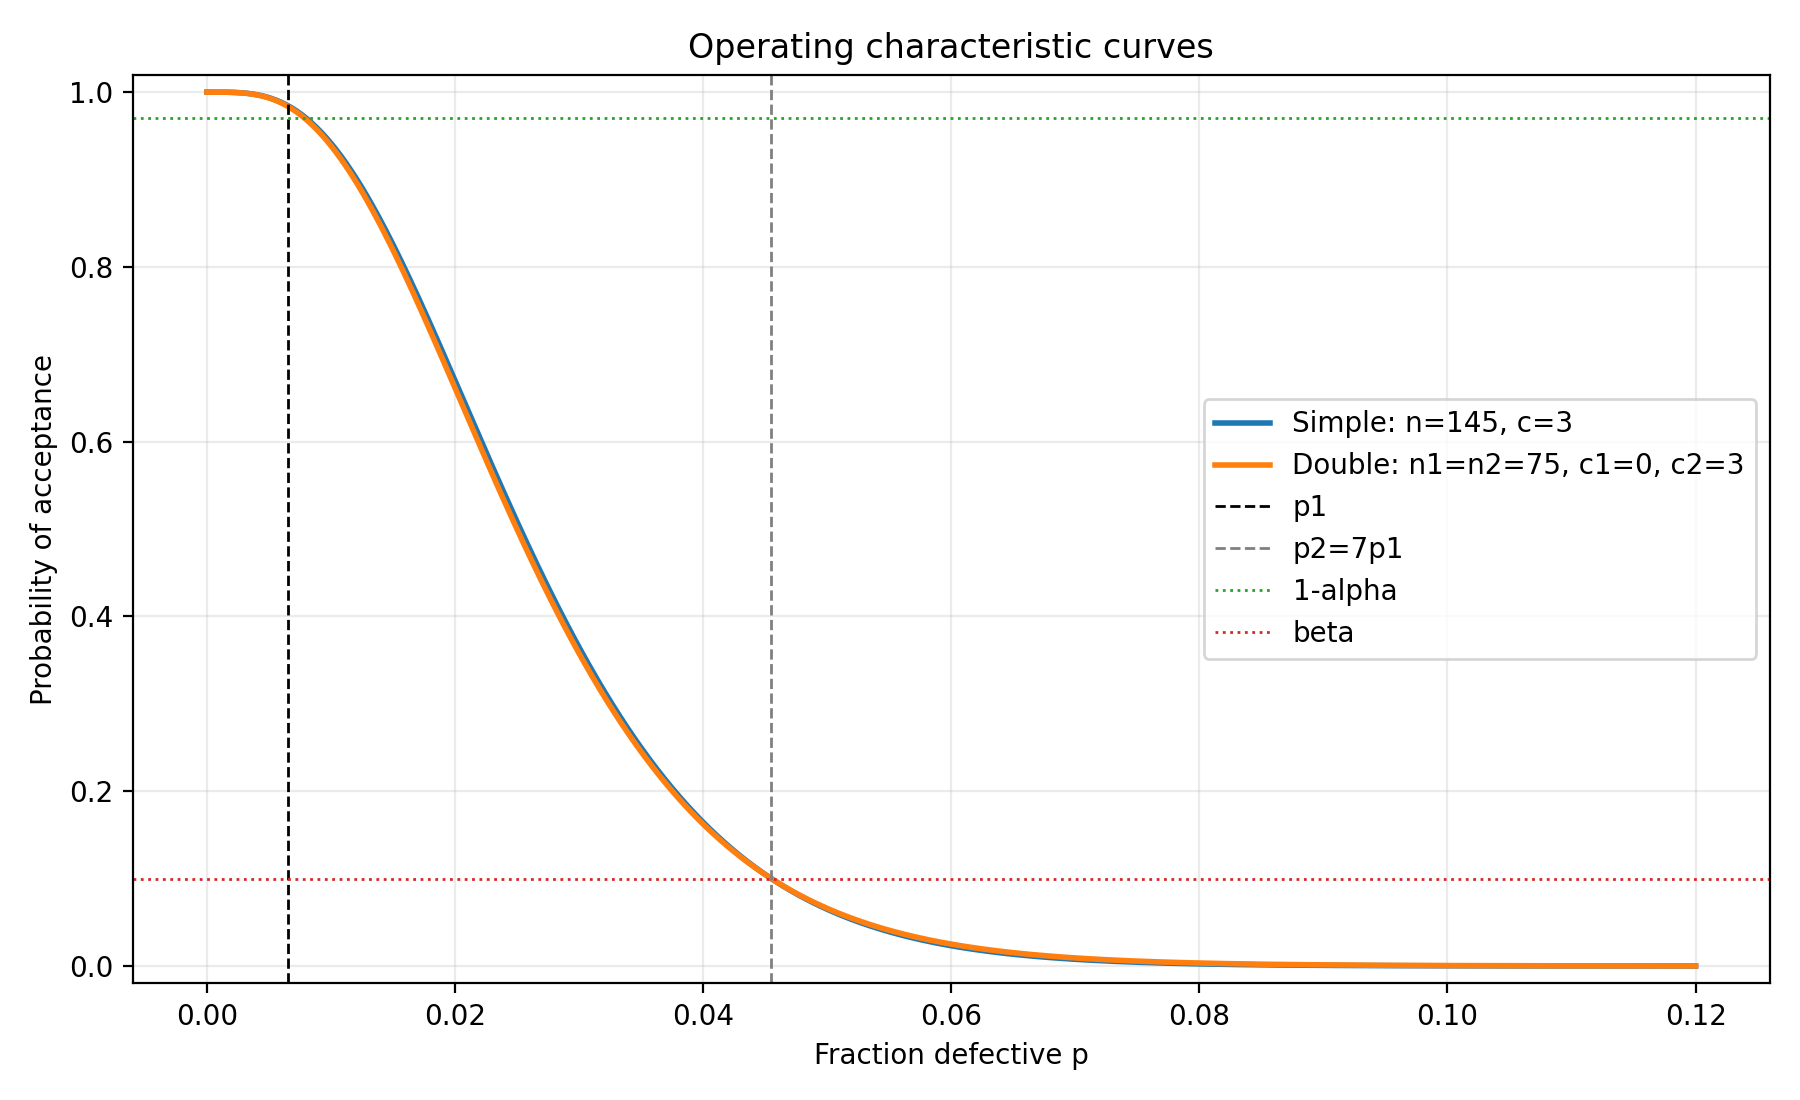
\includegraphics[width=0.92\textwidth]{acceptance_oc_curves.png}
\caption{Χαρακτηριστικές καμπύλες αποδοχής για το απλό και το διπλό σχήμα.}
\label{fig:oc}
\end{figure}

Στο σημείο \(p_1=0{,}0065\), και τα δύο σχήματα έχουν πιθανότητα αποδοχής πάνω
από 0,97. Αυτό σημαίνει ότι οι καλές παρτίδες γίνονται σχεδόν πάντα αποδεκτές.

Στο σημείο \(p_2=0{,}0455\), και τα δύο σχήματα έχουν πιθανότητα αποδοχής
περίπου 0,10. Αυτό σημαίνει ότι οι κακές παρτίδες απορρίπτονται με πιθανότητα
περίπου 90\%.

Οι καμπύλες \(\ATI(p)\) φαίνονται στο Σχήμα~\ref{fig:ati}. Εδώ η διαφορά των
δύο σχημάτων είναι πιο ενδιαφέρουσα.

\begin{figure}[H]
\centering
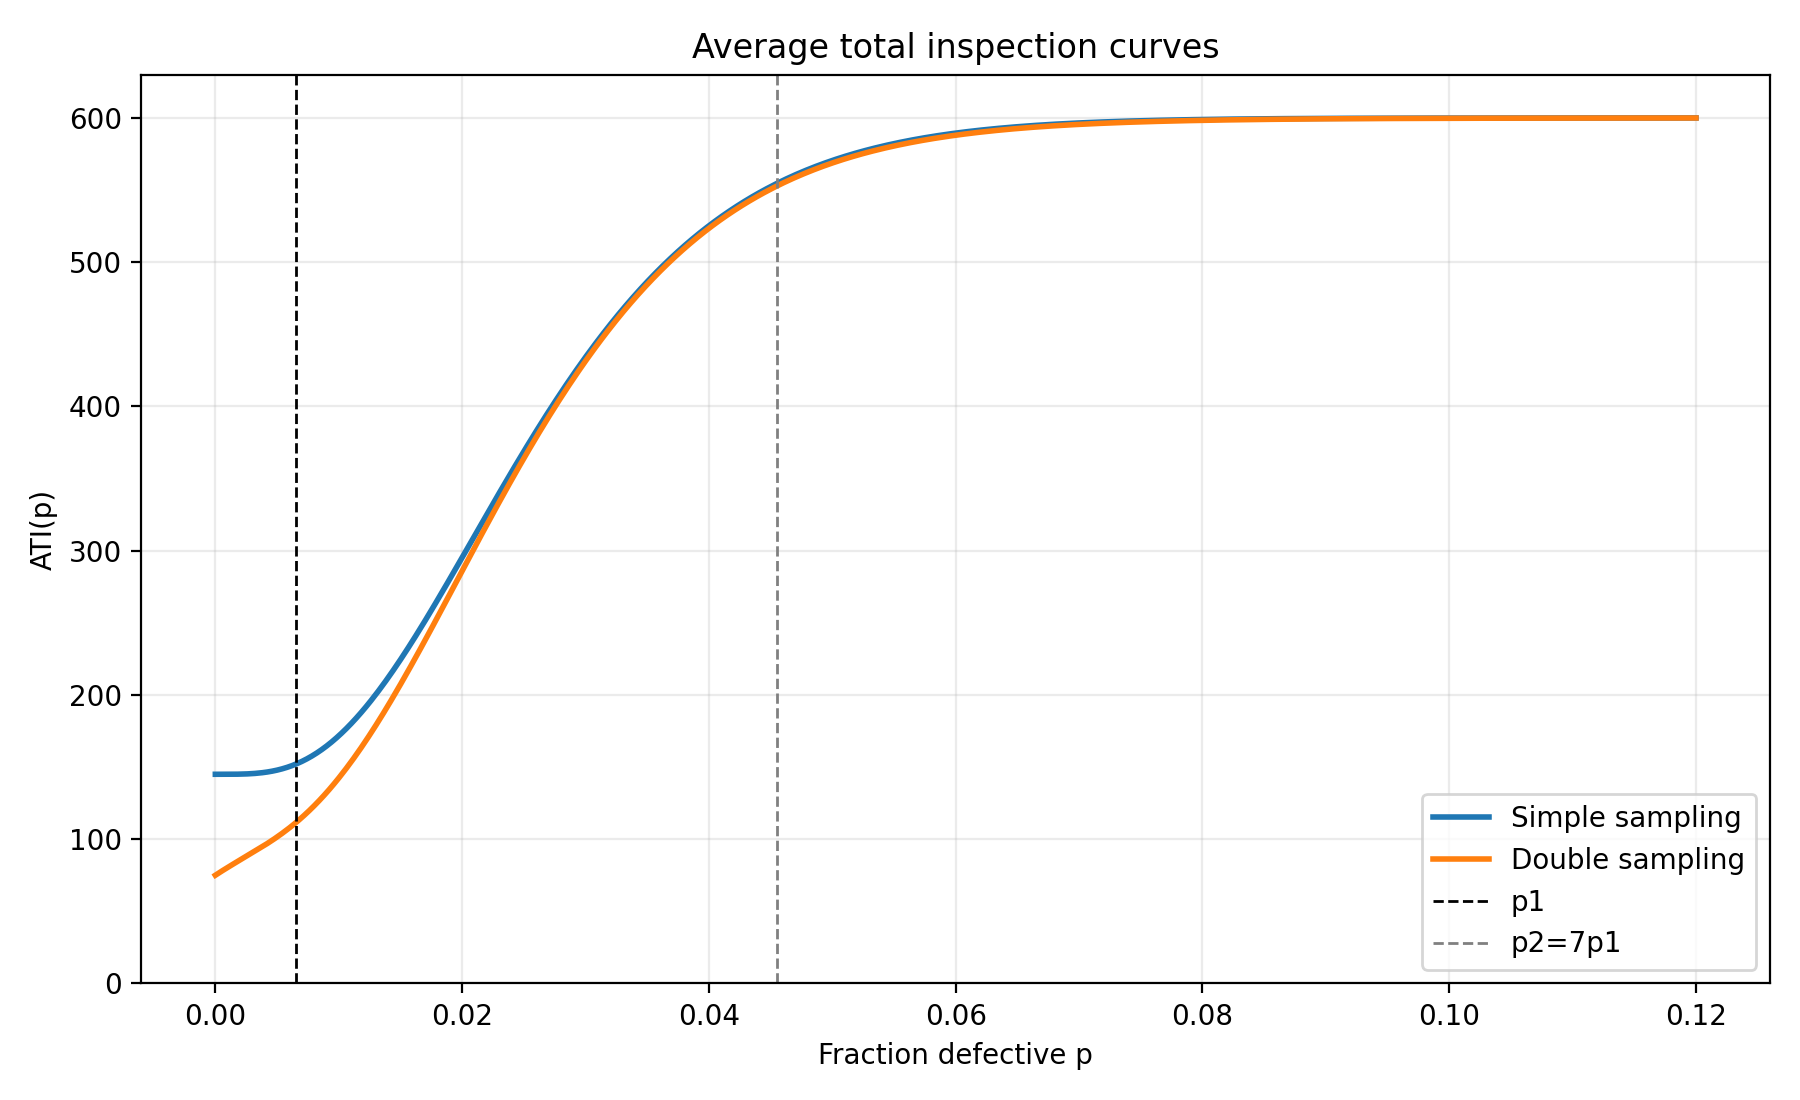
\includegraphics[width=0.92\textwidth]{acceptance_ati_curves.png}
\caption{Μέσος συνολικός αριθμός επιθεωρούμενων μονάδων.}
\label{fig:ati}
\end{figure}

Για πολύ μικρές τιμές του \(p\), το διπλό σχήμα ελέγχει λιγότερες μονάδες κατά
μέσο όρο. Αυτό συμβαίνει επειδή πολλές καλές παρτίδες γίνονται αποδεκτές στο
πρώτο δείγμα των 75 εξαρτημάτων. Αντίθετα, το απλό σχήμα ελέγχει πάντα 145
μονάδες πριν πάρει απόφαση.

Καθώς το \(p\) μεγαλώνει, αυξάνεται η πιθανότητα απόρριψης. Όταν μια παρτίδα
απορρίπτεται, γίνεται πλήρης έλεγχος των 600 μονάδων. Για αυτό και οι δύο
καμπύλες \(\ATI(p)\) ανεβαίνουν και πλησιάζουν το 600.

Στο Σχήμα~\ref{fig:aoq} φαίνονται οι καμπύλες \(\AOQ(p)\). Και οι δύο μένουν
κάτω από το όριο \(3p_1=0{,}0195\), άρα ικανοποιούν τον περιορισμό της
εκφώνησης.

\begin{figure}[H]
\centering
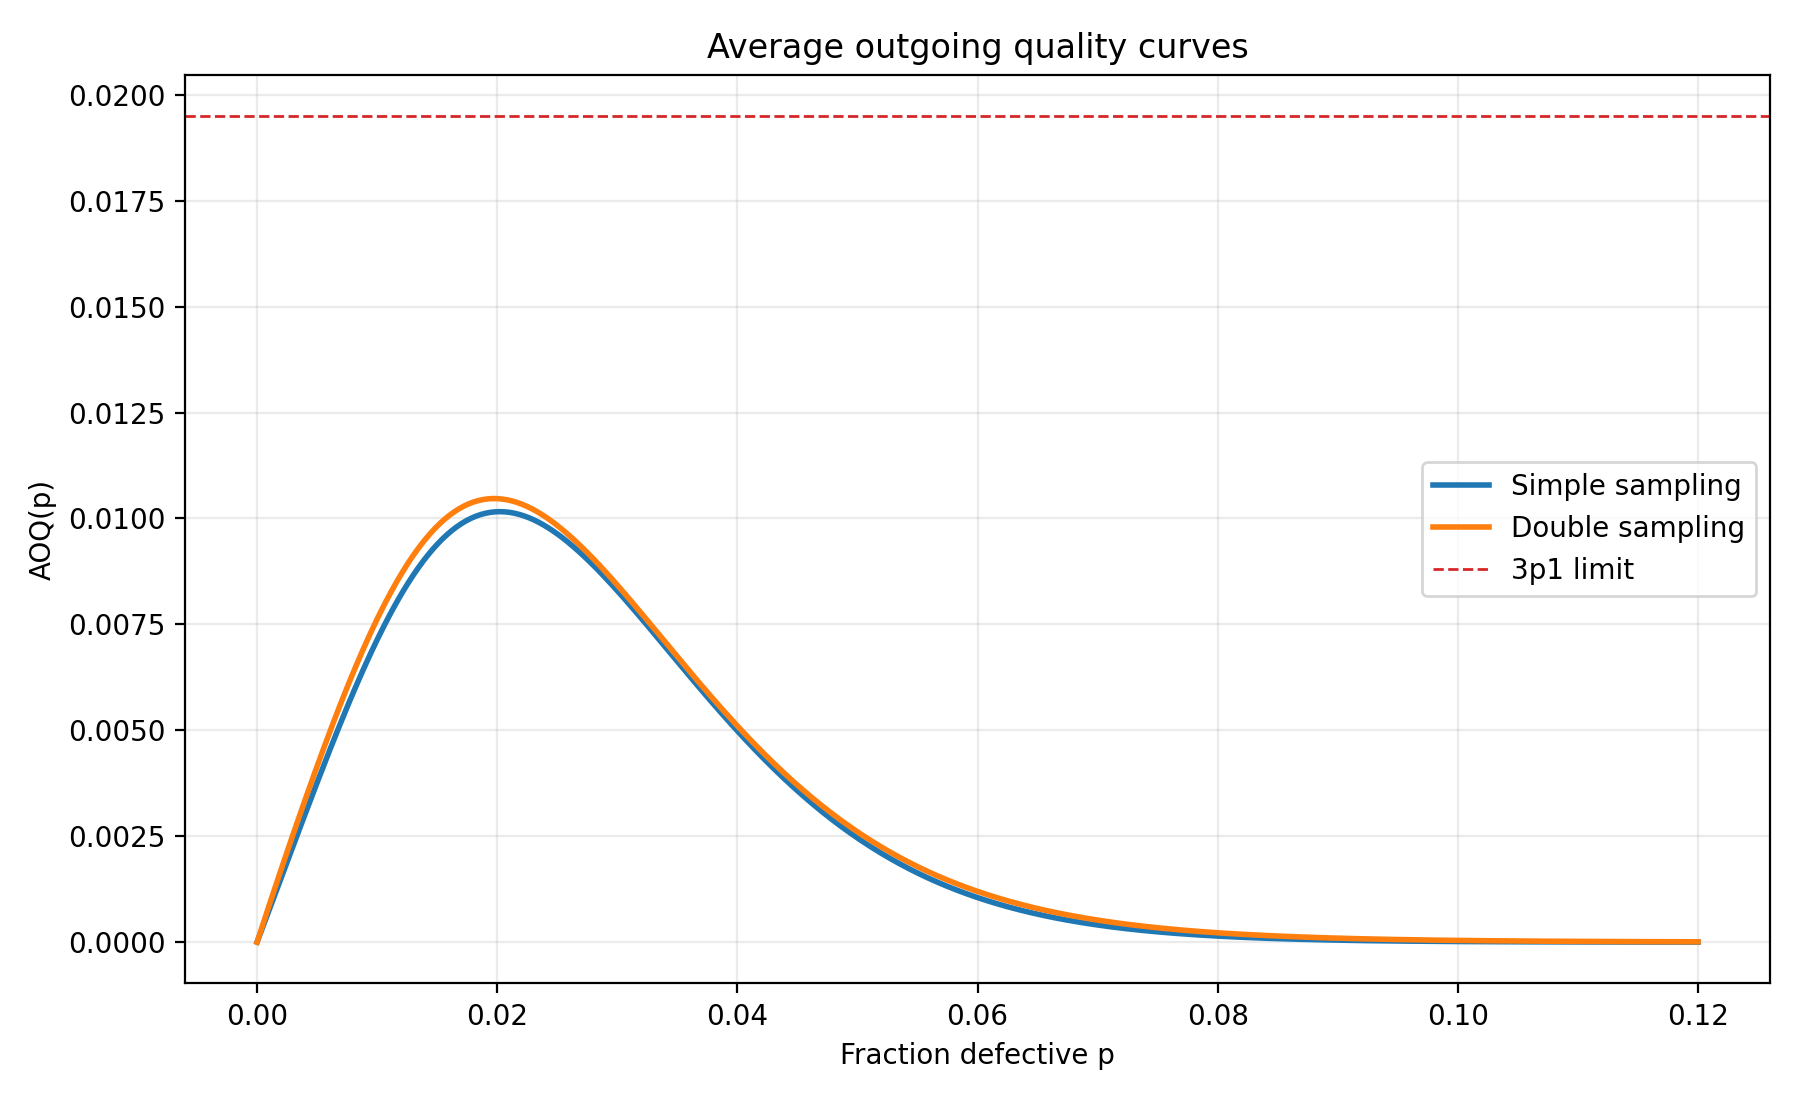
\includegraphics[width=0.92\textwidth]{acceptance_aoq_curves.png}
\caption{Μέση εξερχόμενη ποιότητα και όριο \(3p_1\).}
\label{fig:aoq}
\end{figure}

Το βασικό συμπέρασμα είναι το εξής: τα δύο σχήματα έχουν παρόμοια ικανότητα
διάκρισης καλών και κακών παρτίδων, αλλά το διπλό σχήμα είναι πιο οικονομικό
σε αριθμό ελέγχων όταν η ποιότητα είναι καλή.

%-----------------------------------------------------------------------------
\subsection{Ερώτημα Α4: Βέλτιστο απλό σχήμα ως προς το κόστος}
%-----------------------------------------------------------------------------

\subsubsection*{Τι ζητάει το ερώτημα}

Στα πρώτα ερωτήματα σχεδιάσαμε σχήματα με βάση κινδύνους και ποιότητα. Τώρα η
εκφώνηση αλλάζει κριτήριο και ζητά οικονομική βελτιστοποίηση.

Μας λέει ότι το ποσοστό ελαττωματικών μιας παρτίδας δεν είναι σταθερό. Μπορεί
να θεωρηθεί τυχαίο και να ακολουθεί ομοιόμορφη κατανομή μεταξύ \(p=0{,}004\)
και \(q=0{,}060\).

Ζητά να βρούμε απλό σχήμα με:
\[
    c\le 1,
\]
που ελαχιστοποιεί το μέσο συνολικό κόστος ανά παρτίδα.

\subsubsection*{Θεωρητικό υπόβαθρο}

Το συνολικό κόστος έχει δύο μέρη.

Το πρώτο μέρος είναι το κόστος ελέγχου. Αν κατά μέσο όρο ελέγχουμε
\(\ATI(p)\) εξαρτήματα και κάθε έλεγχος κοστίζει \(c_i\), τότε:
\[
    \text{Κόστος ελέγχου}=c_i\,\ATI(p).
\]

Το δεύτερο μέρος είναι το κόστος των ελαττωματικών που διαφεύγουν. Αν μια
παρτίδα γίνει αποδεκτή, τα εξαρτήματα εκτός δείγματος περνούν στην παραγωγή.
Ο αναμενόμενος αριθμός ελαττωματικών που διαφεύγουν είναι:
\[
    p\,\Pa(p)(N-n).
\]

Αφού κάθε τέτοιο ελαττωματικό κοστίζει \(c_d\), το κόστος τους είναι:
\[
    c_d\,p\,\Pa(p)(N-n).
\]

Άρα το συνολικό κόστος για δεδομένο \(p\) είναι:
\[
    C(p)=c_i\,\ATI(p)+c_d\,p\,\Pa(p)(N-n).
\]

Επειδή το \(p\) είναι τυχαίο και ομοιόμορφο στο διάστημα \([p_L,p_U]\), το
μέσο κόστος είναι:
\[
    E[C]=\frac{1}{p_U-p_L}
    \int_{p_L}^{p_U}C(p)\,dp.
\]

\subsubsection*{Λύση βήμα προς βήμα}

Στην Python δοκιμάστηκαν όλα τα απλά σχήματα με:
\[
    1\le n\le 600,\qquad c=0 \text{ ή } c=1.
\]

Για κάθε σχήμα υπολογίστηκε το μέσο κόστος \(E[C]\). Το μικρότερο κόστος
προέκυψε για:
\[
    \boxed{n=189,\qquad c=1}.
\]

Δηλαδή:

\begin{itemize}
    \item παίρνουμε δείγμα 189 εξαρτημάτων,
    \item αποδεχόμαστε την παρτίδα αν βρούμε 0 ή 1 ελαττωματικό,
    \item απορρίπτουμε την παρτίδα αν βρούμε 2 ή περισσότερα ελαττωματικά.
\end{itemize}

\begin{table}[H]
\centering
\caption{Σύγκριση μέσου συνολικού κόστους.}
\begin{tabular}{lrrr}
\toprule
\textbf{Σχήμα} & \textbf{\(n\)} & \textbf{\(c\)} & \textbf{Μέσο κόστος} \\
\midrule
Βέλτιστο με \(c\le 1\) & 189 & 1 & 3.522,36 € \\
Σχήμα Ερωτήματος Α1 & 145 & 3 & 3.912,03 € \\
\bottomrule
\end{tabular}
\end{table}

Η διαφορά κόστους είναι:
\[
    3.912{,}03-3.522{,}36=389{,}67 \text{ € ανά παρτίδα}.
\]

Σε ποσοστό:
\[
    \frac{389{,}67}{3.522{,}36}\cdot 100=11{,}06\%.
\]

Άρα, με καθαρά οικονομικό κριτήριο και με περιορισμό \(c\le 1\), το σχήμα
\((189,1)\) είναι καλύτερο. Αυτό δεν σημαίνει ότι το σχήμα του Α1 ήταν λάθος.
Το Α1 απαντούσε σε διαφορετικό πρόβλημα: έπρεπε να ικανοποιεί συγκεκριμένους
κινδύνους παραγωγού και πελάτη και περιορισμό \(\AOQL\). Το Α4 ζητά
ελαχιστοποίηση κόστους κάτω από διαφορετικό περιορισμό.

\newpage

%=============================================================================
\section{Μέρος Β: Διαγράμματα ελέγχου}
%=============================================================================

\subsection{Γενική ιδέα του Μέρους Β}

Στο Μέρος Β δεν αποφασίζουμε αν θα αποδεχτούμε ή θα απορρίψουμε μια παρτίδα.
Παρακολουθούμε μια παραγωγική διαδικασία όσο αυτή λειτουργεί. Θέλουμε να
εντοπίσουμε γρήγορα αν συμβεί κάποια συστηματική αιτία που αλλάζει τη
συμπεριφορά της διαδικασίας.

Η τάση εξόδου των τροφοδοτικών πρέπει να είναι κοντά στα 9 V. Όταν η διαδικασία
λειτουργεί κανονικά:
\[
    X\sim N(9,\sigma^2),
\]
με:
\[
    \sigma=0{,}035.
\]

Υπάρχουν δύο πιθανές συστηματικές αιτίες:

\begin{itemize}
    \item μεταβολή της μέσης τάσης κατά \(\Delta=0{,}06\) V,
    \item αύξηση της τυπικής απόκλισης κατά 20\%, δηλαδή από \(\sigma\) σε
    \(1{,}2\sigma\).
\end{itemize}

Για να παρακολουθήσουμε και τις δύο πιθανές αλλαγές, χρησιμοποιούμε δύο
διαγράμματα:

\begin{itemize}
    \item διάγραμμα μέσης τιμής \(\bar X\), για αλλαγές στο κέντρο της
    διαδικασίας,
    \item διάγραμμα τυπικής απόκλισης \(S\), για αλλαγές στη μεταβλητότητα.
\end{itemize}

%-----------------------------------------------------------------------------
\subsection{Ερώτημα Β1: Κατασκευή διαγραμμάτων ελέγχου}
%-----------------------------------------------------------------------------

\subsubsection*{Τι ζητάει το ερώτημα}

Το πρώτο ερώτημα του Μέρους Β ζητά να κατασκευάσουμε απλά διαγράμματα ελέγχου
μέσης τιμής και τυπικής απόκλισης με όρια \(k\) τυπικών αποκλίσεων. Εδώ
\(k=2{,}5\).

Με απλά λόγια, πρέπει να βρούμε:

\begin{itemize}
    \item το κεντρικό όριο και τα δύο όρια ελέγχου για τη δειγματική μέση τιμή,
    \item το κεντρικό όριο και τα δύο όρια ελέγχου για τη δειγματική τυπική
    απόκλιση.
\end{itemize}

\subsubsection*{Θεωρητικό υπόβαθρο για το διάγραμμα μέσης τιμής}

Κάθε ώρα παίρνουμε δείγμα μεγέθους:
\[
    n=5.
\]

Αν η διαδικασία είναι εντός ελέγχου, η δειγματική μέση τιμή \(\bar X\) έχει
μέση τιμή:
\[
    E(\bar X)=\mu_0=9,
\]
και τυπική απόκλιση:
\[
    \sigma_{\bar X}=\frac{\sigma}{\sqrt{n}}.
\]

Άρα τα όρια του διαγράμματος \(\bar X\) είναι:
\[
    LCL_{\bar X}=\mu_0-k\frac{\sigma}{\sqrt n},
\]
\[
    CL_{\bar X}=\mu_0,
\]
\[
    UCL_{\bar X}=\mu_0+k\frac{\sigma}{\sqrt n}.
\]

Η λογική είναι απλή: όσο η διαδικασία είναι κανονική, οι δειγματικές μέσες
τιμές πρέπει να κινούνται γύρω από το 9. Αν κάποια δειγματική μέση τιμή πέσει
εκτός των ορίων, έχουμε ένδειξη ότι η διαδικασία μπορεί να έχει μετατοπιστεί.

\subsubsection*{Υπολογισμός ορίων για το διάγραμμα μέσης τιμής}

Αντικαθιστούμε:
\[
    \mu_0=9,\qquad \sigma=0{,}035,\qquad n=5,\qquad k=2{,}5.
\]

Η τυπική απόκλιση της \(\bar X\) είναι:
\[
    \frac{0{,}035}{\sqrt 5}=0{,}015652.
\]

Άρα:
\[
    2{,}5\cdot 0{,}015652=0{,}039131.
\]

Επομένως:
\[
    LCL_{\bar X}=9-0{,}039131=8{,}960869,
\]
\[
    UCL_{\bar X}=9+0{,}039131=9{,}039131.
\]

\subsubsection*{Θεωρητικό υπόβαθρο για το διάγραμμα τυπικής απόκλισης}

Το διάγραμμα \(S\) παρακολουθεί τη μεταβλητότητα της διαδικασίας. Αν η
μεταβλητότητα μεγαλώσει, τότε τα δείγματα θα έχουν μεγαλύτερες τυπικές
αποκλίσεις.

Η δειγματική τυπική απόκλιση \(S\) δεν έχει μέση τιμή ακριβώς ίση με
\(\sigma\). Για κανονικά δεδομένα:
\[
    E(S)=c_4\sigma,
\]
όπου \(c_4\) είναι σταθερά που εξαρτάται από το μέγεθος δείγματος.

Για \(n=5\):
\[
    c_4=
    \sqrt{\frac{2}{n-1}}
    \frac{\Gamma(n/2)}{\Gamma((n-1)/2)}
    =0{,}939986.
\]

Η τυπική απόκλιση του \(S\) είναι:
\[
    \sigma_S=\sigma\sqrt{1-c_4^2}.
\]

Άρα τα όρια του διαγράμματος \(S\) είναι:
\[
    LCL_S=\max(0,c_4\sigma-k\sigma_S),
\]
\[
    CL_S=c_4\sigma,
\]
\[
    UCL_S=c_4\sigma+k\sigma_S.
\]

Χρησιμοποιούμε το \(\max(0,\cdot)\), επειδή η τυπική απόκλιση δεν μπορεί να
είναι αρνητική.

\subsubsection*{Υπολογισμός ορίων για το διάγραμμα τυπικής απόκλισης}

Με \(\sigma=0{,}035\) και \(c_4=0{,}939986\):
\[
    CL_S=c_4\sigma=0{,}939986\cdot 0{,}035=0{,}032899.
\]

Η τυπική απόκλιση του \(S\) είναι:
\[
    \sigma_S=0{,}011942.
\]

Άρα:
\[
    LCL_S=0{,}032899-2{,}5\cdot 0{,}011942=0{,}003043,
\]
\[
    UCL_S=0{,}032899+2{,}5\cdot 0{,}011942=0{,}062756.
\]

\begin{table}[H]
\centering
\caption{Τελικά όρια διαγραμμάτων ελέγχου.}
\begin{tabular}{lrrr}
\toprule
\textbf{Διάγραμμα} & \textbf{LCL} & \textbf{CL} & \textbf{UCL} \\
\midrule
\(\bar X\) & 8,960869 & 9,000000 & 9,039131 \\
\(S\) & 0,003043 & 0,032899 & 0,062756 \\
\bottomrule
\end{tabular}
\end{table}

%-----------------------------------------------------------------------------
\subsection{Ερώτημα Β2: Πιθανότητα σφάλματος πρώτου είδους}
%-----------------------------------------------------------------------------

\subsubsection*{Τι ζητάει το ερώτημα}

Το δεύτερο ερώτημα ζητά την πιθανότητα σφάλματος πρώτου είδους. Στο πλαίσιο
διαγραμμάτων ελέγχου, σφάλμα πρώτου είδους σημαίνει ότι το διάγραμμα δίνει
σήμα εκτός ελέγχου ενώ στην πραγματικότητα η διαδικασία είναι εντός ελέγχου.

Με απλά λόγια, είναι η πιθανότητα ψευδούς συναγερμού.

Επειδή έχουμε δύο διαγράμματα, το ερώτημα ζητά την πιθανότητα να δώσει
εσφαλμένη ένδειξη είτε το διάγραμμα \(\bar X\), είτε το διάγραμμα \(S\), είτε
και τα δύο.

\subsubsection*{Θεωρητικό υπόβαθρο}

Για το διάγραμμα \(\bar X\), όταν η διαδικασία είναι εντός ελέγχου, η
τυποποιημένη δειγματική μέση τιμή ακολουθεί τυπική κανονική κατανομή:
\[
    Z=\frac{\bar X-\mu_0}{\sigma/\sqrt n}\sim N(0,1).
\]

Τα όρια είναι στις \(k=2{,}5\) τυπικές αποκλίσεις, άρα:
\[
    \alpha_{\bar X}=P(|Z|>2{,}5).
\]

Για το διάγραμμα \(S\), χρησιμοποιούμε το γεγονός ότι:
\[
    \frac{(n-1)S^2}{\sigma^2}\sim \chi^2_{n-1}.
\]

Αυτή η σχέση μας επιτρέπει να υπολογίσουμε ακριβώς την πιθανότητα το \(S\) να
πέσει κάτω από το \(LCL_S\) ή πάνω από το \(UCL_S\).

Για κανονικά δεδομένα, η \(\bar X\) και το \(S\) είναι ανεξάρτητα. Επομένως η
πιθανότητα να μη δώσει κανένα διάγραμμα ψευδή ένδειξη είναι:
\[
    (1-\alpha_{\bar X})(1-\alpha_S).
\]

Άρα η πιθανότητα να δώσει τουλάχιστον ένα διάγραμμα ψευδή ένδειξη είναι:
\[
    \alpha_{\text{ολ}}=
    1-(1-\alpha_{\bar X})(1-\alpha_S).
\]

\subsubsection*{Λύση βήμα προς βήμα}

Για το διάγραμμα \(\bar X\):
\[
    \alpha_{\bar X}=2[1-\Phi(2{,}5)].
\]

Από την κανονική κατανομή:
\[
    \alpha_{\bar X}=0{,}012419.
\]

Για το διάγραμμα \(S\), με την κατανομή \(\chi^2_4\):
\[
    \alpha_S=0{,}012095.
\]

Άρα:
\[
    \alpha_{\text{ολ}}=
    1-(1-0{,}012419)(1-0{,}012095).
\]

Τελικό αποτέλεσμα:
\[
    \boxed{\alpha_{\text{ολ}}=0{,}024364}.
\]

Δηλαδή, ακόμη και όταν η διαδικασία λειτουργεί κανονικά, υπάρχει περίπου
2,44\% πιθανότητα σε ένα χρονικό σημείο να πάρουμε ψευδή ένδειξη από ένα από
τα δύο διαγράμματα.

%-----------------------------------------------------------------------------
\subsection{Ερώτημα Β3: Ισχύς του διαγράμματος μέσης τιμής}
%-----------------------------------------------------------------------------

\subsubsection*{Τι ζητάει το ερώτημα}

Το τρίτο ερώτημα ζητά την ισχύ του διαγράμματος \(\bar X\) όταν η μέση τιμή
μεταβληθεί από 9 σε:
\[
    9+\Delta
    \quad \text{ή} \quad
    9-\Delta.
\]

Επειδή \(\Delta=0{,}06\), η νέα μέση τιμή γίνεται είτε \(9{,}06\) είτε
\(8{,}94\).

Η ισχύς είναι η πιθανότητα να καταλάβει το διάγραμμα ότι κάτι άλλαξε. Δηλαδή
είναι η πιθανότητα το \(\bar X\) να πέσει εκτός ορίων μετά τη μετατόπιση της
μέσης τιμής.

Το ερώτημα ζητά αυτή την ισχύ σε δύο περιπτώσεις:

\begin{itemize}
    \item όταν αλλάζει μόνο η μέση τιμή,
    \item όταν αλλάζει η μέση τιμή και ταυτόχρονα αυξάνεται η τυπική απόκλιση
    κατά 20\%.
\end{itemize}

\subsubsection*{Θεωρητικό υπόβαθρο}

Τα όρια ελέγχου έχουν υπολογιστεί με βάση την κανονική κατάσταση της
διαδικασίας. Αν όμως η πραγματική μέση τιμή γίνει \(\mu_1=9+\Delta\), τότε:
\[
    \bar X\sim N\left(\mu_1,\frac{\sigma'^2}{n}\right),
\]
όπου \(\sigma'\) είναι η πραγματική τυπική απόκλιση μετά τη μεταβολή.

Η ισχύς είναι:
\[
    P(\bar X<LCL_{\bar X})+
    P(\bar X>UCL_{\bar X}).
\]

Λόγω συμμετρίας, η μεταβολή προς τα κάτω κατά \(\Delta\) δίνει ίδια ισχύ με τη
μεταβολή προς τα πάνω κατά \(\Delta\).

\subsubsection*{Λύση βήμα προς βήμα}

Τα όρια του διαγράμματος \(\bar X\) είναι:
\[
    LCL_{\bar X}=8{,}960869,\qquad
    UCL_{\bar X}=9{,}039131.
\]

Αν η μέση τιμή γίνει \(9{,}06\) και η τυπική απόκλιση μείνει \(\sigma=0{,}035\),
τότε η πιθανότητα ένδειξης εκτός ελέγχου είναι:
\[
    \boxed{0{,}908777}.
\]

Αν η μέση τιμή γίνει \(9{,}06\) και ταυτόχρονα η τυπική απόκλιση γίνει
\(1{,}2\sigma\), τότε η ισχύς γίνεται:
\[
    \boxed{0{,}866727}.
\]

\begin{table}[H]
\centering
\caption{Ισχύς του διαγράμματος μέσης τιμής.}
\begin{tabular}{lr}
\toprule
\textbf{Περίπτωση} & \textbf{Ισχύς} \\
\midrule
Μεταβολή μέσης τιμής, χωρίς αύξηση \(\sigma\) & 0,908777 \\
Μεταβολή μέσης τιμής, με αύξηση \(\sigma\) κατά 20\% & 0,866727 \\
\bottomrule
\end{tabular}
\end{table}

Η ισχύς είναι υψηλή, επειδή η μετατόπιση \(0{,}06\) V είναι αρκετά μεγάλη σε
σχέση με την τυπική απόκλιση της δειγματικής μέσης τιμής. Η παράλληλη αύξηση
της μεταβλητότητας μειώνει λίγο την ισχύ για αυτή τη συγκεκριμένη μετατόπιση,
επειδή η κατανομή της \(\bar X\) απλώνεται περισσότερο γύρω από τη νέα μέση
τιμή.

%-----------------------------------------------------------------------------
\subsection{Ερώτημα Β4: Ισχύς του διαγράμματος τυπικής απόκλισης}
%-----------------------------------------------------------------------------

\subsubsection*{Τι ζητάει το ερώτημα}

Το τέταρτο ερώτημα ζητά την ισχύ του διαγράμματος \(S\) όταν η τυπική απόκλιση
αυξηθεί από:
\[
    \sigma
    \quad \text{σε} \quad
    1{,}2\sigma.
\]

Το ζητά και σε δύο περιπτώσεις:

\begin{itemize}
    \item χωρίς παράλληλη μεταβολή της μέσης τιμής,
    \item με παράλληλη μεταβολή της μέσης τιμής.
\end{itemize}

\subsubsection*{Θεωρητικό υπόβαθρο}

Το διάγραμμα \(S\) δεν κοιτάει πού βρίσκεται το κέντρο της διαδικασίας. Κοιτάει
πόσο απλωμένες είναι οι τιμές μέσα στο δείγμα. Για κανονικά δεδομένα, η
κατανομή του \(S\) εξαρτάται από την τυπική απόκλιση \(\sigma\), αλλά όχι από
τη μέση τιμή \(\mu\).

Άρα, αν αλλάξει μόνο η μέση τιμή, το διάγραμμα \(S\) δεν επηρεάζεται. Αν όμως
αλλάξει η τυπική απόκλιση, τότε το \(S\) τείνει να παίρνει μεγαλύτερες τιμές
και μπορεί να ξεπεράσει το άνω όριο ελέγχου.

Η ισχύς είναι:
\[
    P(S<LCL_S \text{ ή } S>UCL_S\mid \sigma'=1{,}2\sigma).
\]

\subsubsection*{Λύση βήμα προς βήμα}

Με:
\[
    LCL_S=0{,}003043,\qquad UCL_S=0{,}062756,
\]
και νέα τυπική απόκλιση:
\[
    \sigma'=1{,}2\sigma=1{,}2\cdot 0{,}035=0{,}042,
\]
η πιθανότητα ένδειξης εκτός ελέγχου είναι:
\[
    \boxed{0{,}062919}.
\]

Επειδή η κατανομή του \(S\) δεν εξαρτάται από τη μέση τιμή, η ίδια τιμή ισχύει
και όταν υπάρχει παράλληλη μετατόπιση της μέσης τιμής.

\begin{table}[H]
\centering
\caption{Ισχύς του διαγράμματος τυπικής απόκλισης.}
\begin{tabular}{lr}
\toprule
\textbf{Περίπτωση} & \textbf{Ισχύς} \\
\midrule
Αύξηση \(\sigma\) κατά 20\%, χωρίς μεταβολή μέσης τιμής & 0,062919 \\
Αύξηση \(\sigma\) κατά 20\%, με μεταβολή μέσης τιμής & 0,062919 \\
\bottomrule
\end{tabular}
\end{table}

Η ισχύς είναι σχετικά μικρή. Αυτό σημαίνει ότι με δείγματα μεγέθους 5 και
όρια \(2{,}5\) τυπικών αποκλίσεων, το διάγραμμα \(S\) δεν είναι ιδιαίτερα
ευαίσθητο σε αύξηση της τυπικής απόκλισης μόνο κατά 20\%.

%-----------------------------------------------------------------------------
\subsection{Ερώτημα Β5: Κόστος κακής ποιότητας μέχρι την ανίχνευση}
%-----------------------------------------------------------------------------

\subsubsection*{Τι ζητάει το ερώτημα}

Το πέμπτο ερώτημα συνδέει τον στατιστικό έλεγχο με οικονομικό κόστος. Μας λέει
να υπολογίσουμε το μέσο κόστος κακής ποιότητας από τη στιγμή που αλλάζει η μέση
τιμή μέχρι τη στιγμή που το διάγραμμα \(\bar X\) ανιχνεύει αυτή την αλλαγή.

Η τυπική απόκλιση θεωρείται ότι δεν αλλάζει σε αυτό το διάστημα.

\subsubsection*{Θεωρητικό υπόβαθρο}

Αν η μέση τιμή μετατοπιστεί, τότε κάποια προϊόντα θα βγαίνουν εκτός
προδιαγραφών. Τα όρια προδιαγραφών είναι:
\[
    LSL=8{,}90,\qquad USL=9{,}10.
\]

Αν μετά τη μετατόπιση έχουμε:
\[
    X\sim N(9{,}06,\;0{,}035^2),
\]
τότε η πιθανότητα ελαττωματικού προϊόντος είναι:
\[
    P(X<8{,}90)+P(X>9{,}10).
\]

Αυτό δεν είναι πιθανότητα σήματος από το διάγραμμα. Είναι πιθανότητα να
παραχθεί ελαττωματικό προϊόν.

Αφού η παραγωγή είναι 100 τροφοδοτικά ανά ώρα, ο αναμενόμενος αριθμός
ελαττωματικών ανά ώρα είναι:
\[
    100\cdot P(\text{ελαττωματικό}).
\]

Κάθε ελαττωματικό κοστίζει \(K=21\) €, άρα το κόστος ανά ώρα είναι:
\[
    100\cdot P(\text{ελαττωματικό})\cdot 21.
\]

Τώρα χρειαζόμαστε και τον μέσο χρόνο μέχρι να ανιχνευθεί η μεταβολή. Αν η
πιθανότητα ανίχνευσης σε κάθε δείγμα είναι \(\pi\), τότε ο μέσος αριθμός
δειγμάτων μέχρι την ένδειξη είναι:
\[
    ARL_1=\frac{1}{\pi}.
\]

Εδώ \(\pi\) είναι η ισχύς του διαγράμματος \(\bar X\) από το Ερώτημα Β3.

\subsubsection*{Λύση βήμα προς βήμα}

Η πιθανότητα ελαττωματικού μετά τη μετατόπιση της μέσης τιμής είναι:
\[
    P(X<8{,}90)+P(X>9{,}10)=0{,}126551.
\]

Άρα περίπου το 12,6551\% των τροφοδοτικών θα είναι εκτός προδιαγραφών όσο η
διαδικασία παραμένει σε αυτή τη μετατοπισμένη κατάσταση.

Το κόστος κακής ποιότητας ανά ώρα είναι:
\[
    0{,}126551\cdot 100\cdot 21=265{,}76 \text{ €/ώρα}.
\]

Η πιθανότητα ανίχνευσης της μεταβολής σε κάθε δείγμα είναι:
\[
    \pi=0{,}908777.
\]

Άρα:
\[
    ARL_1=\frac{1}{0{,}908777}=1{,}10038.
\]

Επειδή παίρνουμε ένα δείγμα ανά ώρα, αυτό σημαίνει ότι αν η μεταβολή συμβεί
ακριβώς μετά από μια δειγματοληψία, ο μέσος χρόνος μέχρι την ένδειξη είναι:
\[
    1{,}10038 \text{ ώρες}.
\]

Το αντίστοιχο κόστος είναι:
\[
    265{,}76\cdot 1{,}10038=292{,}43 \text{ €}.
\]

Στην πράξη, μια μεταβολή μπορεί να συμβεί σε τυχαία στιγμή μέσα στο διάστημα
μεταξύ δύο δειγματοληψιών. Τότε, κατά μέσο όρο, χάνεται μισή ώρα λιγότερη,
επειδή η μεταβολή δεν συμβαίνει πάντα ακριβώς μετά από δείγμα. Ο μέσος χρόνος
μέχρι την ένδειξη είναι:
\[
    ARL_1-\frac{1}{2}=1{,}10038-0{,}5=0{,}60038 \text{ ώρες}.
\]

Άρα το μέσο κόστος κακής ποιότητας είναι:
\[
    265{,}76\cdot 0{,}60038
    =
    \boxed{159{,}56 \text{ €}}.
\]

Συνοψίζοντας:

\begin{table}[H]
\centering
\caption{Κόστος κακής ποιότητας μέχρι την ανίχνευση της μετατόπισης.}
\begin{tabular}{lr}
\toprule
\textbf{Υπόθεση για τη στιγμή μεταβολής} & \textbf{Μέσο κόστος} \\
\midrule
Μεταβολή σε τυχαία στιγμή μέσα στο ωριαίο διάστημα & 159,56 € \\
Μεταβολή αμέσως μετά από δειγματοληψία & 292,43 € \\
\bottomrule
\end{tabular}
\end{table}

Η πρώτη τιμή είναι η πιο ρεαλιστική όταν δεν γνωρίζουμε πότε ακριβώς συμβαίνει
η συστηματική αιτία. Η δεύτερη είναι πιο συντηρητική, γιατί υποθέτει τη
χειρότερη χρονική θέση μέσα στον κύκλο δειγματοληψίας.

%-----------------------------------------------------------------------------
\subsection{Ερώτημα Β6: Έλεγχος των 15 πραγματικών δειγμάτων}
%-----------------------------------------------------------------------------

\subsubsection*{Τι ζητάει το ερώτημα}

Το τελευταίο ερώτημα μάς δίνει 15 δείγματα, καθένα με 5 μετρήσεις τάσης. Ζητά
να αποφασίσουμε αν η διαδικασία ήταν σε στατιστικό έλεγχο κατά τη διάρκεια
λήψης αυτών των δειγμάτων.

Με απλά λόγια:

\begin{itemize}
    \item Υπολογίζουμε τη μέση τιμή κάθε δείγματος.
    \item Υπολογίζουμε την τυπική απόκλιση κάθε δείγματος.
    \item Βάζουμε τις τιμές στα δύο διαγράμματα ελέγχου.
    \item Αν κάποια τιμή βγει εκτός ορίων, έχουμε ένδειξη ότι η διαδικασία δεν
    ήταν σε στατιστικό έλεγχο.
\end{itemize}

\subsubsection*{Θεωρητικό υπόβαθρο}

Μια διαδικασία είναι σε στατιστικό έλεγχο όταν η μεταβλητότητά της μπορεί να
αποδοθεί μόνο σε τυχαίες, φυσιολογικές αιτίες. Δεν σημαίνει ότι όλα τα προϊόντα
είναι τέλεια. Σημαίνει ότι η διαδικασία είναι σταθερή και προβλέψιμη.

Αν όμως δούμε σημεία εκτός ορίων ελέγχου, τότε υπάρχει ένδειξη ειδικής ή
συστηματικής αιτίας. Σε αυτή την περίπτωση δεν λέμε ότι η διαδικασία είναι
στατιστικά ελεγχόμενη.

\subsubsection*{Λύση βήμα προς βήμα}

Για κάθε ένα από τα 15 δείγματα υπολογίστηκαν:
\[
    \bar x=\frac{x_1+x_2+x_3+x_4+x_5}{5},
\]
και η δειγματική τυπική απόκλιση:
\[
    s=\sqrt{\frac{\sum_{i=1}^{5}(x_i-\bar x)^2}{5-1}}.
\]

Στη συνέχεια οι τιμές συγκρίθηκαν με τα όρια:
\[
    8{,}960869\le \bar x\le 9{,}039131,
\]
\[
    0{,}003043\le s\le 0{,}062756.
\]

\begin{longtable}{rrrrl}
\caption{Έλεγχος των 15 δειγμάτων με βάση τα διαγράμματα \(\bar X\) και \(S\).}
\label{tab:samples}\\
\toprule
\textbf{Δείγμα} & \textbf{\(\bar x\)} & \textbf{\(s\)} & \textbf{Εκτός \(\bar X\)} & \textbf{Συμπέρασμα} \\
\midrule
\endfirsthead
\toprule
\textbf{Δείγμα} & \textbf{\(\bar x\)} & \textbf{\(s\)} & \textbf{Εκτός \(\bar X\)} & \textbf{Συμπέρασμα} \\
\midrule
\endhead
1 & 8,992 & 0,04087 & Όχι & Εντός ελέγχου \\
2 & 9,018 & 0,03033 & Όχι & Εντός ελέγχου \\
3 & 9,012 & 0,02775 & Όχι & Εντός ελέγχου \\
4 & 9,024 & 0,04506 & Όχι & Εντός ελέγχου \\
5 & 8,984 & 0,01140 & Όχι & Εντός ελέγχου \\
6 & 9,006 & 0,02302 & Όχι & Εντός ελέγχου \\
7 & 8,980 & 0,05148 & Όχι & Εντός ελέγχου \\
8 & 9,012 & 0,03271 & Όχι & Εντός ελέγχου \\
9 & 9,004 & 0,04930 & Όχι & Εντός ελέγχου \\
10 & 9,058 & 0,04087 & Ναι & Εκτός ελέγχου \\
11 & 9,086 & 0,03362 & Ναι & Εκτός ελέγχου \\
12 & 9,070 & 0,00707 & Ναι & Εκτός ελέγχου \\
13 & 9,038 & 0,04207 & Όχι & Εντός ελέγχου \\
14 & 9,066 & 0,03715 & Ναι & Εκτός ελέγχου \\
15 & 9,072 & 0,04147 & Ναι & Εκτός ελέγχου \\
\bottomrule
\end{longtable}

Το διάγραμμα φαίνεται στο Σχήμα~\ref{fig:charts}. Τα κόκκινα σημεία στο
διάγραμμα \(\bar X\) είναι οι ενδείξεις εκτός ελέγχου.

\begin{figure}[H]
\centering
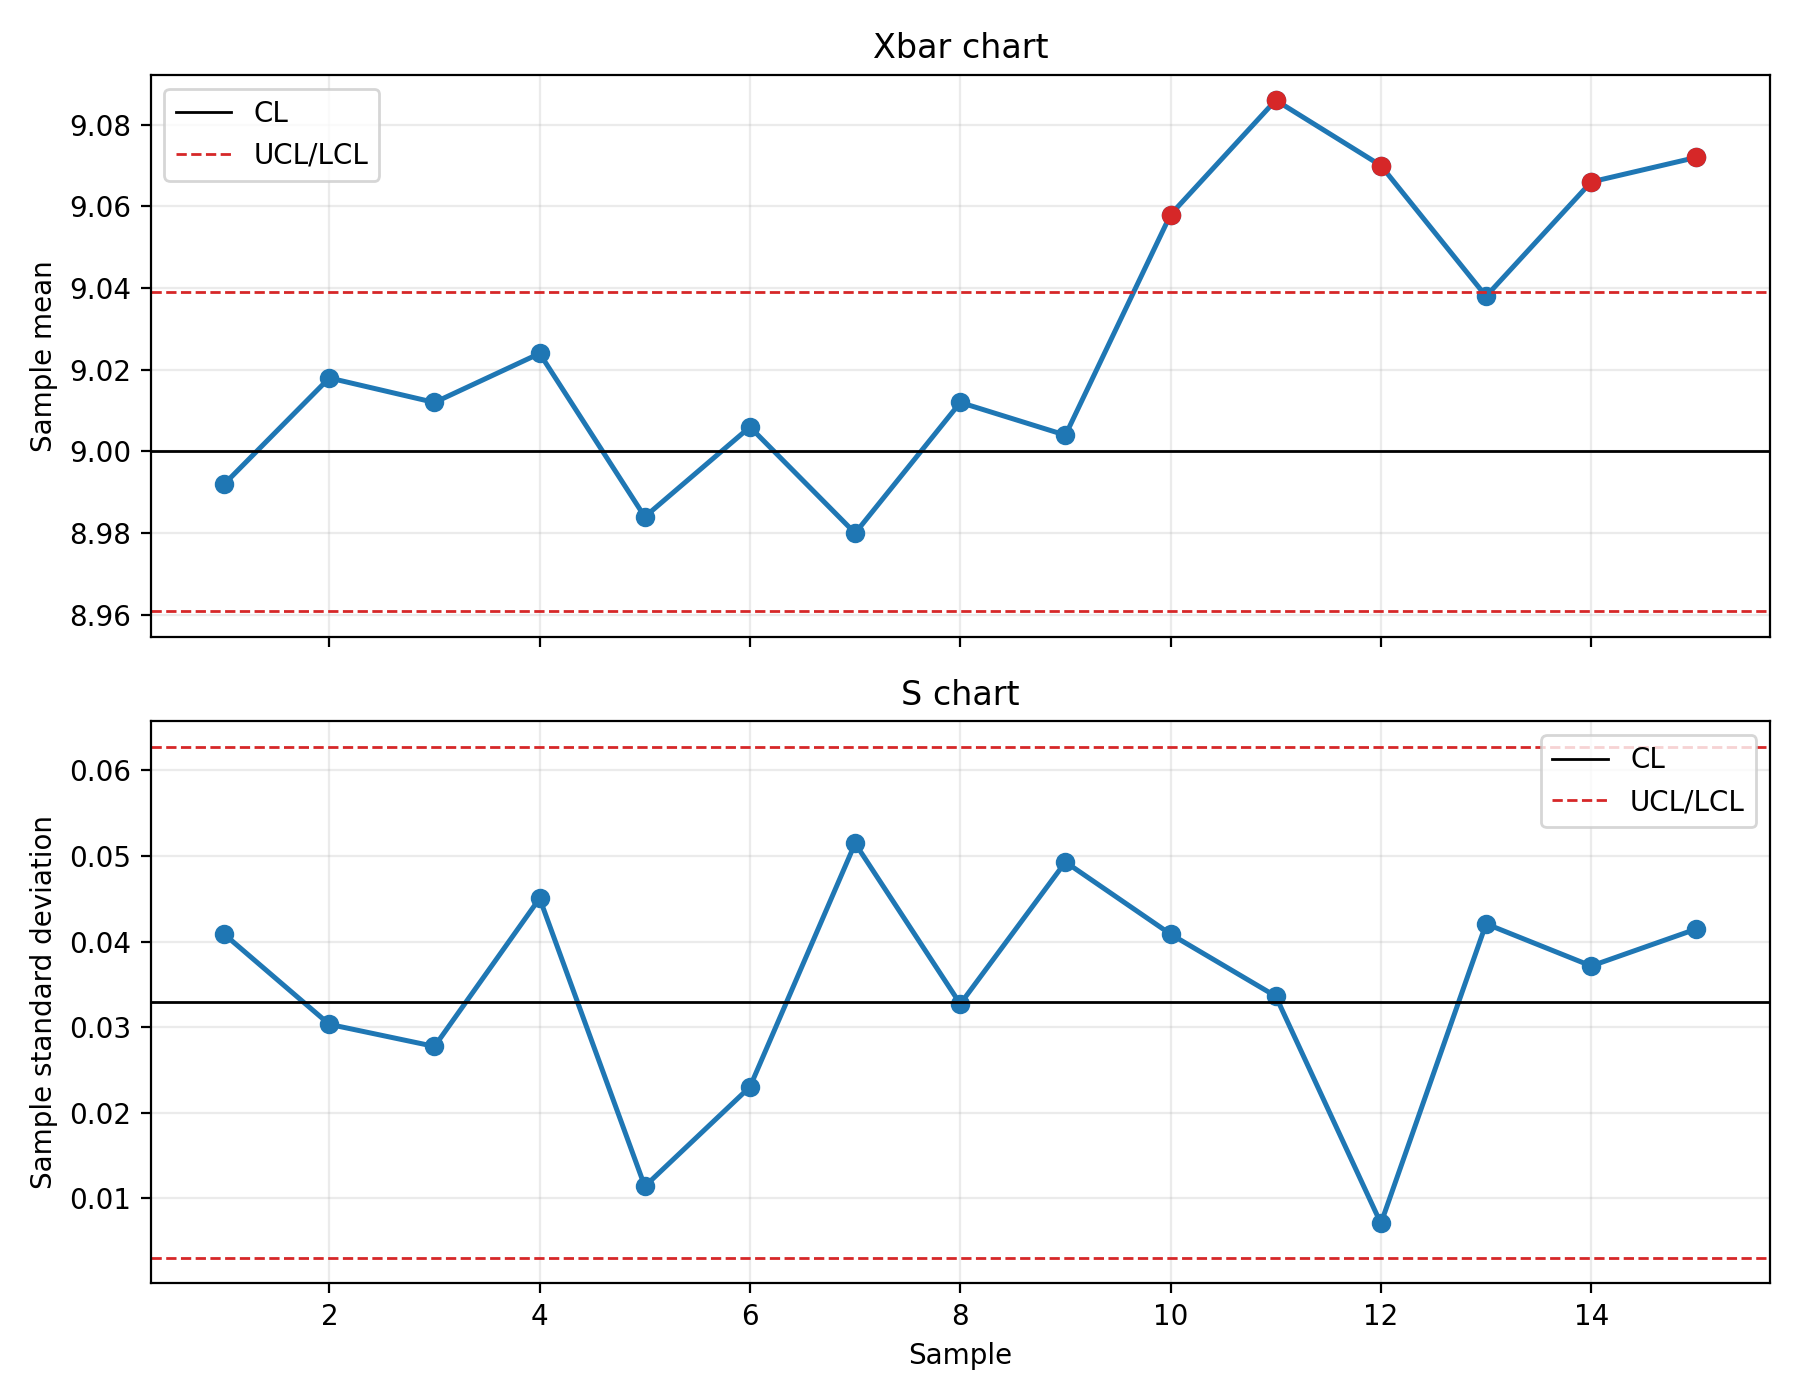
\includegraphics[width=0.92\textwidth]{control_charts_samples.png}
\caption{Διαγράμματα \(\bar X\) και \(S\) για τα 15 δείγματα.}
\label{fig:charts}
\end{figure}

Τα δείγματα που είναι εκτός ελέγχου στο διάγραμμα μέσης τιμής είναι:
\[
    10,\ 11,\ 12,\ 14,\ 15.
\]

Κανένα δείγμα δεν είναι εκτός ελέγχου στο διάγραμμα \(S\). Αυτό είναι πολύ
χρήσιμο ως ερμηνεία. Μας λέει ότι το πρόβλημα δεν φαίνεται να είναι αύξηση της
μεταβλητότητας. Το πρόβλημα φαίνεται να είναι μετατόπιση της μέσης τιμής προς
τα πάνω.

Άρα το τελικό συμπέρασμα είναι:

\begin{center}
\fbox{\begin{minipage}{0.88\textwidth}
\centering
Η διαδικασία δεν ήταν σε στατιστικό έλεγχο κατά τη διάρκεια των 15 δειγμάτων.
\end{minipage}}
\end{center}

Πιο συγκεκριμένα, από το δείγμα 10 και μετά εμφανίζεται ένδειξη ότι η μέση
τάση έχει αυξηθεί.

\newpage

%=============================================================================
\section{Τελική σύνοψη}
%=============================================================================

Στο Μέρος Α μάθαμε πώς σχεδιάζεται ένας δειγματοληπτικός έλεγχος αποδοχής.
Το απλό σχήμα που ικανοποιεί τους κινδύνους παραγωγού και πελάτη και τον
περιορισμό \(\AOQL\) είναι:
\[
    \boxed{(n,c)=(145,3)}.
\]

Το διπλό σχήμα με \(c_1=0\), ίσα μεγέθη δειγμάτων και συνολικό μέγιστο δείγμα
μεγαλύτερο από 145 είναι:
\[
    \boxed{(n_1,n_2,c_1,c_2)=(75,75,0,3)}.
\]

Οι χαρακτηριστικές καμπύλες των δύο σχημάτων είναι παρόμοιες, επειδή και τα
δύο σχεδιάστηκαν για τις ίδιες απαιτήσεις στα σημεία \(p_1\) και \(p_2\). Όμως
το διπλό σχήμα μπορεί να απαιτεί λιγότερους ελέγχους όταν η ποιότητα είναι
καλή.

Στο οικονομικό ερώτημα, με περιορισμό \(c\le 1\), το βέλτιστο απλό σχήμα είναι:
\[
    \boxed{(n,c)=(189,1)}.
\]

Το μέσο κόστος του είναι 3.522,36 € ανά παρτίδα, ενώ το σχήμα του Α1 έχει μέσο
κόστος 3.912,03 € ανά παρτίδα.

Στο Μέρος Β κατασκευάστηκαν τα διαγράμματα ελέγχου:
\[
    \bar X: \quad 8{,}960869 \le \bar X \le 9{,}039131,
\]
\[
    S: \quad 0{,}003043 \le S \le 0{,}062756.
\]

Η συνολική πιθανότητα ψευδούς ένδειξης από ένα τουλάχιστον διάγραμμα είναι:
\[
    \boxed{0{,}024364}.
\]

Η ισχύς του διαγράμματος \(\bar X\) για μετατόπιση της μέσης τιμής κατά
0,06 V είναι υψηλή:
\[
    \boxed{0{,}908777}.
\]

Αντίθετα, η ισχύς του διαγράμματος \(S\) για αύξηση της τυπικής απόκλισης κατά
20\% είναι χαμηλή:
\[
    \boxed{0{,}062919}.
\]

Στα 15 πραγματικά δείγματα, τα δείγματα 10, 11, 12, 14 και 15 βγήκαν εκτός
ελέγχου από το διάγραμμα \(\bar X\), ενώ κανένα δείγμα δεν βγήκε εκτός ελέγχου
από το διάγραμμα \(S\). Άρα η διαδικασία δεν ήταν σε στατιστικό έλεγχο και η
ένδειξη αφορά κυρίως μετατόπιση της μέσης τάσης προς τα πάνω.

\end{document}
